\section{example}
\begin{frame}{problem }
  \begin{figure}[htbq]
    \centering
    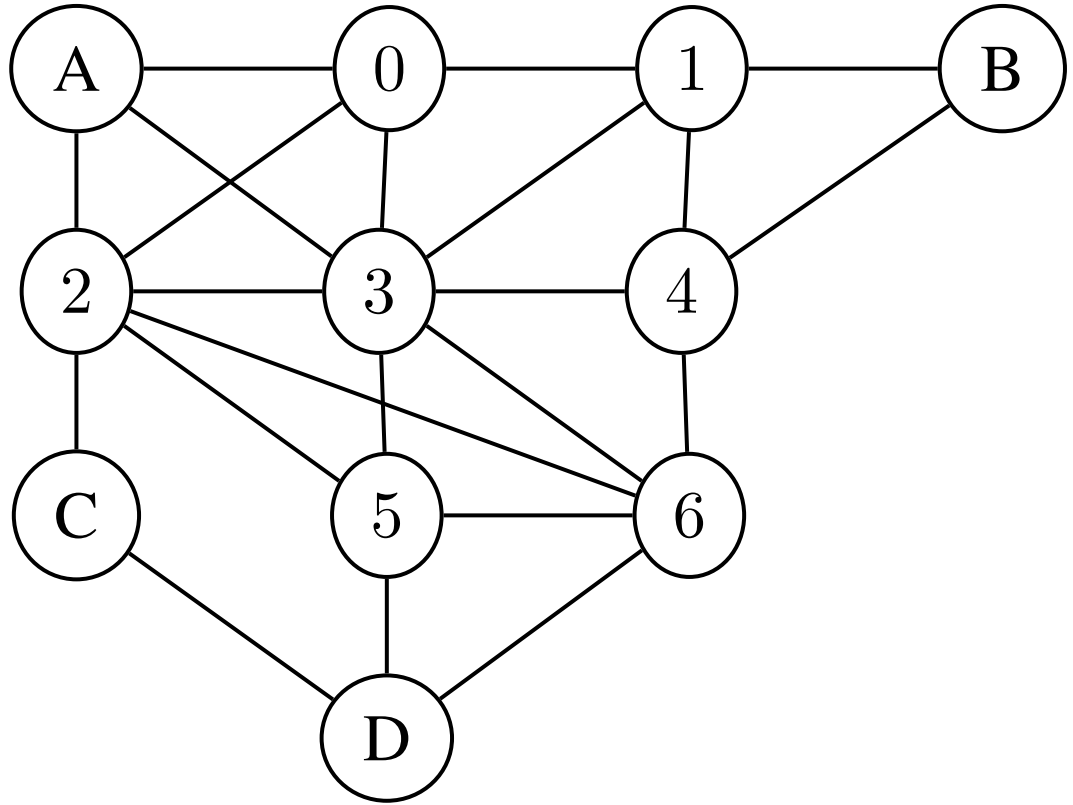
\includegraphics[width=0.5\textwidth]{figure/problem.png}
    \caption{Zed city as an undirected graph} 
    \label{fig-zed}
  \end{figure}
\end{frame}
\begin{frame}[fragile]
  \frametitle{initial state boolean function}
  \begin{block}{python implementation of initial function f}
    \begin{lstlisting}[language=Python]
def g(v0, ..., v6 : BitVec(2)) -> BitVec(1):
  return (v0 != ’00’) and (v1 != ’01’) and(v2 != ’00’) and (v2 != ’10’) and(v3 != ’00’) and (v4 != ’01’) and(v5 != ’11’) and (v6 != ’11’)
    \end{lstlisting}
  \end{block}
\end{frame}

\begin{frame}[fragile]
  \frametitle{boolean function}
  \begin{columns}
    \begin{column}{0.45\linewidth}
      \begin{block}{python implementation of f }
        \begin{lstlisting}[language=Python]
def f(v0, ..., v6 : BitVec(2)) -> BitVec(1):
  c0 = (v0 != ’00’)
  c1 = (v1 != ’01’) and (v1 != v0)
  c2 = (v2 != ’00’) and (v2 != ’10’) and (v2 != v0)
  c3 = (v3 != ’00’) and (v3 != v0) and (v3 != v1) and (v3 != v2)
  c4 = (v4 != ’01’) and (v4 != v1) and (v4 != v3)
  c5 = (v5 != ’11’) and (v5 != v2) and (v5 != v3)
  c6 = (v6 != ’11’) and (v6 != v2) and (v6 != v3) and (v6 != v4) and (v6 != v5)
  return c0 and c1 and c2 and c3 and c4 and c5 and c6
          \end{lstlisting}
      \end{block}
    \end{column}
    \begin{column}{0.45\linewidth}
      \begin{block}{hand-optimized python implementation of f }
        \begin{lstlisting}[language=Python]
def f(v0, ..., v6 : BitVec(2)) -> BitVec(1):
  c1 = (v1[0] == v1[1]) and (v3 != v1)
  c023 = ((v0 ˆ v2 ˆ v3) == ’00’)
  c4 = (v4 != v1) and (v4 != v3)
  c5 = (v5 != v2) and (v5 != v3)
  c6 = ((v2 ˆ v3 ˆ v5 ˆ v6) == ’00’) and (v6 != v4)
  return c1 and c023 and c4 and c5 and c6
          \end{lstlisting}
      \end{block}
    \end{column}
  \end{columns}
\end{frame}


\begin{frame}{result\footfullcite{example}}
  \begin{table}[htbq]
    \begin{tabular}{@{}ccccc@{}}
    \toprule
    \multirow{2}{*}{} & \multicolumn{2}{c}{\text { Hand-optimized }} & \multicolumn{2}{c}{\text { Non-optimized }} \\ \cmidrule(l){2-5} 
                      &  \text { Qubits } & \text { cost } & \text { Qubits } & \text { cost } \\ \hline
    \text { IBM's solution } & 32 & 5004 & & \\
    \text { Whit3z solution } & 32 & 2474 & & \\
    \text { XAG-based flow } & 31 & 2202 & 56 & 4347 \\
    \text { XAG-based flow with pebbling } & 21 & 4497  & 30 & 7737 \\
    \bottomrule
    \end{tabular}
    \caption{quality  of results for boolean function (hand-optimized and non-optimized), where $cost = q_1+10q_2$}
  \end{table}  
\end{frame}
